%!TEX root = Pflichtenheft.tex

\section{Benutzeroberfläche}

\subsection{Kommando-Struktur}
Die Kommando-Struktur der Benutzeroberfläche ist durch das Program \emph{git} inspiriert\\
\\\\
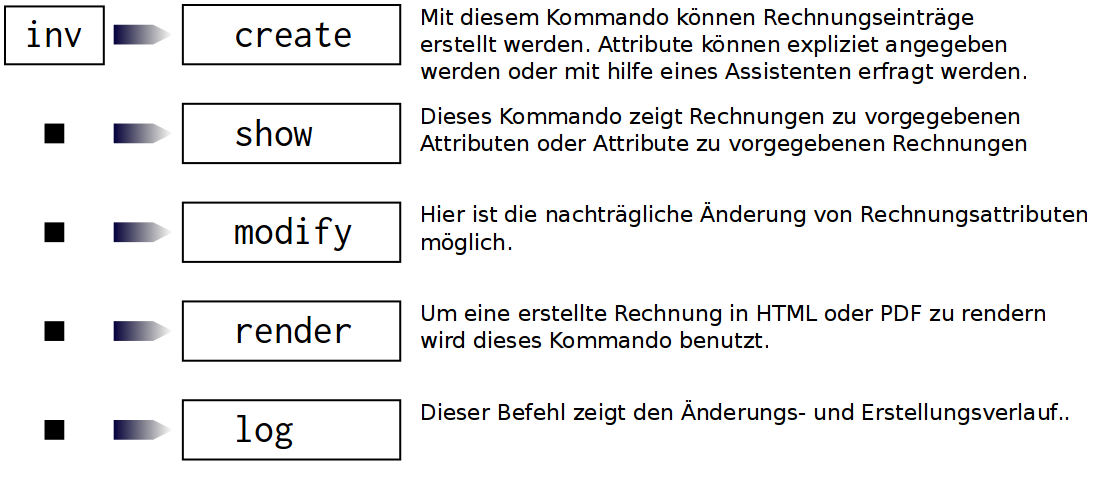
\includegraphics[width=\textwidth]{kommando-struktur.png}
\\
\\
\subsection{Ordnerstruktur}
Es ist möglich mit der Ordnerstruktur innerhalb eines Repositories diverse
Standard-Attributwerte zu definieren. Dies geschieht im Zusammen mit den vom
Benutzer gewählten Ordnungsschlüsseln.\\
\\\\
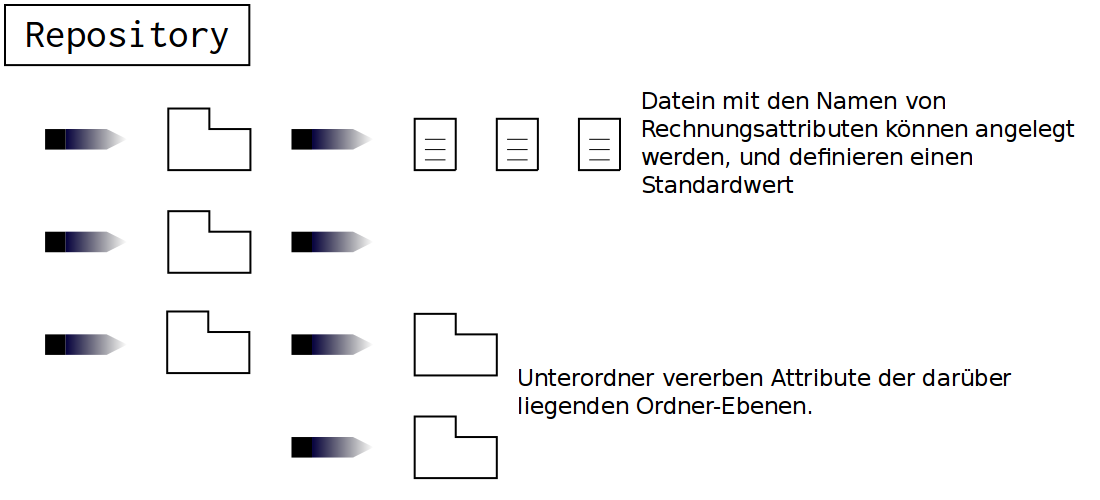
\includegraphics[width=\textwidth]{ordnerstruktur-struktur.png}



